% V6 Paper — Ensemble Tabular Q-Learning for Pokemon Battling
% Author: Arzaan Singh, Tulane University
% Advisor: Dr. Zizhan Zheng
%
% Build: pdflatex main && bibtex main && pdflatex main && pdflatex main
% Or with latexmk: latexmk -pdf main
%
% NOTE: Download neurips_2024.sty from https://neurips.cc/Conferences/2024/PaperInformation/StyleFiles
% and place it in this directory before compiling.

\documentclass{article}

% NeurIPS style file (uncomment after placing neurips_2024.sty in this dir)
% Use [final] for camera-ready, [preprint] for arXiv preprint
\usepackage[preprint]{neurips_2024}

% Standard math + graphics packages
\usepackage{amsmath, amssymb, amsthm}
\usepackage{graphicx}
\usepackage{booktabs}        % Professional tables
\usepackage{siunitx}         % Aligned numbers in tables
\usepackage{microtype}       % Better justification
\usepackage[utf8]{inputenc}
\usepackage[T1]{fontenc}
\usepackage{xcolor}
\usepackage{hyperref}        % Last before cleveref
\usepackage[capitalize,noabbrev]{cleveref}
\usepackage{algorithm}
\usepackage{algorithmic}

% Color setup matching the figure palette (Tulane green primary)
\definecolor{tulanegreen}{HTML}{006747}
\definecolor{tulaneblue}{HTML}{418FDE}
\definecolor{guidered}{HTML}{B00020}
\hypersetup{
  colorlinks=true,
  linkcolor=tulanegreen,
  citecolor=tulanegreen,
  urlcolor=tulaneblue,
}

% Outline guide macro. Renders red italic text inline; intended as a
% short reminder of what the prose in this paragraph should accomplish.
% Use \guide{...} for inline reminders, \guideblock{...} for a paragraph
% block. Both will be stripped once the prose pass replaces them.
\newcommand{\guide}[1]{{\color{guidered}\itshape [#1]}}
\newcommand{\guideblock}[1]{\par\begingroup\color{guidered}\itshape\noindent#1\par\endgroup}

% Title
\title{Ensembling Tabular Q-Learning Agents for Competitive Pokemon\\
  A Read-Only Inference Method with Heuristic-Prior Fallback}

% Author: Arzaan is the sole author of this paper. Zizhan Zheng is the
% research advisor and is acknowledged via a footnote on the author line
% (NeurIPS template convention via \thanks{}). His name does NOT appear
% on the author line itself.
\author{
  Arzaan Singh\thanks{Research advisor: Dr.\ Zizhan Zheng, Department of
  Computer Science, Tulane University (zzheng3@tulane.edu).
  Prof.\ Zheng supervises this research line but is not an author of
  this paper.} \\
  Department of Computer Science \\
  Tulane University \\
  New Orleans, LA \\
  \texttt{singharzaan@gmail.com}
}

\begin{document}

\maketitle

\begin{abstract}
% Abstract — write LAST, after Friday's meeting fixes the contribution framing.
% Target ~200 words. Each \guide{} below marks one sentence in the final draft.

\guide{Sentence 1 (setup): single-agent tabular RL hits a ceiling effect in
stochastic, partially-observable two-player games; Pokemon (gen4ou) is the
benchmark.}

\guide{Sentence 2 (method): we train $K$ independent tabular $Q(\lambda)$
agents under identical hyperparameters but different random seeds and
combine them at inference time using a read-only voting rule with a
heuristic-prior fallback for unseen state-action pairs (no Q-table
mutation at evaluation time).}

\guide{Sentence 3 (headline): $K=10$ ensemble reaches $66.8\% \pm 0.3\%$
win rate vs.\ \texttt{SimpleHeuristicsPlayer} over $100{,}000$ battles,
$+12.6$ pp over a compute-matched single-agent baseline trained for the
same total simulated-battle budget.}

\guide{Sentence 4 (analysis): the $K$-saturation curve has the
Osband-style concave-up shape and plateaus by $K{=}10$; voting rule
(soft / hard / confidence-weighted) has only a small effect at fixed
$K$.}

\guide{Sentence 5 (significance): first Q-function-ensemble study on
Pokemon; the read-only inference rule is the load-bearing methodological
contribution and is independent of the underlying value-function class.}

\end{abstract}

% Section 1: Introduction (~1 page, ~700 words)
% Structure: motivation -> ensembling-specifically -> what's new -> contributions list -> result preview
% Write THIRD, after Method and Results.

\section{Introduction}
\label{sec:introduction}

TODO write after Method + Results exist.

% Paragraph 1 — motivation (5 sentences)
% Tabular RL ceilings, Pokemon as testbed, ~10^12 states, existing single-agent results plateau.

% Paragraph 2 — why ensembling (3 sentences)
% Cite Wiering 2008, Osband 2016, Lan 2020; identify the gap (tabular action-time voting on stochastic adversarial games).

% Paragraph 3 — what's new (2 sentences leading into contributions)

% Contribution list (bulleted, 4 items)
% C1 — Read-only memory-bounded inference rule with heuristic-prior fallback
% C2 — Three-rule voting comparison at K in {1,3,5,10} (first on a non-toy domain)
% C3 — Compute-matched evaluation framework
% C4 — Open-source pipeline

% Result preview (1 sentence + headline number)
% 66.8% vs heuristic, +12.6pp over 5M baseline, z = 62 sigma.

% Paper layout sentence

% Section 2: Related Work (~1 page, ~750 words)
% Outline only — prose pass deferred. Three subsections, ~250 words each.

\section{Related Work}
\label{sec:related_work}

\subsection{Ensemble methods in tabular reinforcement learning}
\label{sec:rw_tabular}

\guideblock{One paragraph. Walk through the tabular ensemble line:
\citet{wiering2008} (first systematic study of voting rules in
$Q$-learning), \citet{fausser2011} (ensemble methods with function
approximation), \citet{lan2020maxmin} (maxmin $Q$-learning as
ensemble-style estimation-bias control), \citet{peer2021ebql} (ensemble
bootstrapping for $Q$-learning). The distinction this paper draws: prior
tabular ensemble work either lives in toy gridworld / small MDP regimes
\emph{or} uses algorithmic diversity (different update rules per member);
we use seed-only diversity in a non-toy stochastic two-player game.}

\subsection{Ensemble methods in deep reinforcement learning}
\label{sec:rw_deep}

\guideblock{One paragraph. Cover the deep-RL ensemble line:
\citet{osband2016bootstrapped} (bootstrapped DQN, posterior-sampling
exploration), \citet{anschel2017avgdqn} (averaged DQN for variance
reduction), \citet{chen2021redq} (randomized ensembled double
$Q$-learning), \citet{lee2021sunrise} (unified ensemble framework).
Close with the \citet{lin2024curse} ``Curse of Diversity'' failure mode:
deep ensembles sharing a replay buffer can underperform their own
single-agent baseline. Set up the contrast: our independent-table setup
has no shared buffer and is shown to be immune by construction (full
discussion in Section~\ref{sec:d_curse}).}

\subsection{Reinforcement learning for Pokemon}
\label{sec:rw_pokemon}

\guideblock{One paragraph in roughly chronological order:
\citet{lee2017showdown} (early Showdown AI competition),
\citet{kalose2018} (Stanford project, early Pokemon RL writeup),
\citet{sahovic2020pokeenv} (\texttt{poke-env}, the library used here),
\citet{simoes2020} (deep RL on the Showdown simulator),
\citet{wang2024mit} (MIT M.Eng.\ thesis on random-battle RL),
\citet{hu2024pokellmon} (LLM-as-policy approach),
\citet{karten2025pokechamp} (expert-level minimax LM agent),
\citet{grigsby2025metamon} (transformer offline RL),
\citet{vgcbench2025} (VGC team-strategy benchmark). Close with the gap
this paper addresses: to our knowledge, no prior paper trains $K$
independent tabular $Q$-function agents under identical hyperparameters
and combines them by inference-time voting on Pokemon battles.}

% Section 3: Background and Method (~1.5 pages, ~1500 words)
% Write FIRST. This defines the technical contribution; everything else flows from it.

\section{Background and Method}
\label{sec:method}

\subsection{Preliminaries}
\label{sec:prelim}

% Define MDP/POMDP notation, Watkins Q(lambda), Pokemon Showdown as POMDP,
% hierarchical action decomposition (20-tuple master state, 17-tuple sub-state),
% heuristic prior h(s, a).

We model a Pokemon battle as a partially observable Markov decision process (POMDP)
$(\mathcal{S}, \mathcal{A}, P, r, \gamma, \Omega)$ where $\mathcal{S}$ is the set of
joint game states, $\mathcal{A}$ is the player's action set (move 1 through 4, plus a
switch action), $P$ is a stochastic transition function determined by the Showdown
simulator, $r$ is the dense reward (HP delta, faint delta, terminal $\pm 1$),
$\gamma$ is the discount factor, and $\Omega : \mathcal{S} \to \mathcal{O}$ is the
observation function that hides opponent team information.

We train each member with Watkins $Q(\lambda)$ \citep{watkins1989, sutton2018}:
\begin{align}
  \delta_t       &= r_{t+1} + \gamma \max_{a'} Q(s_{t+1}, a') - Q(s_t, a_t) \\
  e_t(s, a)      &= \begin{cases} 1, & (s, a) = (s_t, a_t) \\
                                  \gamma \lambda \, e_{t-1}(s, a), & a_t = \arg\max_{a'} Q(s_t, a') \\
                                  0, & \text{otherwise} \end{cases} \\
  Q(s, a)        &\leftarrow Q(s, a) + \alpha \delta_t \, e_t(s, a)
\end{align}
with replacing traces and the trace cleared after non-greedy exploration.

% Hierarchical decomposition (from V5)
We adopt the hierarchical action decomposition introduced in our prior work
\citep{singh2026v5}: a \emph{master} agent observes a 20-tuple state and chooses
between attacking (one of four moves) and switching; if it chooses to switch,
a \emph{sub-agent} observes a 17-tuple state and selects which Pokemon to switch to.
Both agents are trained jointly via the shared reward signal. We use the master's
Q-table $Q^{\text{m}}$ and the sub-agent's Q-table $Q^{\text{s}}$ throughout.

% Heuristic prior h(s, a)
For unseen state-action pairs at inference time, we use the same domain heuristic
$h(s, a)$ that V5 used to ``smart-initialize'' the Q-tables: it is a deterministic
function of the battle state, combining type effectiveness, STAB, move power, and
accuracy. Crucially, $h(s, a)$ depends only on $s$ and the action's type signature,
not on any trained Q-table.

\subsection{The ensemble inference rule}
\label{sec:method_inference}

% This is the technical contribution. State formally.
% Define: Q-matrix at decision time, three combination rules, read-only property.

Given $K$ trained Q-tables $\{Q^k_{\text{m}}, Q^k_{\text{s}}\}_{k=1}^K$, we choose
the agent's action at state $s$ as follows.

\paragraph{Action enumeration.}
Following the master/sub-agent decomposition, we first enumerate the possible
\emph{master} actions $\mathcal{A}_{\text{m}}(s)$ available at state $s$
(legal moves of the active Pokemon, plus a switch action when force-switch is not
required). We then construct the \emph{Q-matrix} $\mathbf{Q} \in \mathbb{R}^{K \times |\mathcal{A}_{\text{m}}|}$
whose entry $\mathbf{Q}_{k, a}$ is the master Q-value of action $a$ at state $s$ under
member $k$, with heuristic fallback for unseen entries:
\begin{equation}
  \mathbf{Q}_{k, a} := \begin{cases}
    Q^k_{\text{m}}(s, a), & \text{if } (s, a) \in \text{dom}(Q^k_{\text{m}}) \\
    h(s, a),              & \text{otherwise.}
  \end{cases}
  \label{eq:q_matrix}
\end{equation}

\paragraph{Combination rules.}
We compare three rules for combining the $K$ rows of $\mathbf{Q}$ into a single
chosen action $a^* \in \mathcal{A}_{\text{m}}$.

\textbf{Soft voting} averages Q-values column-wise and picks the argmax:
\begin{equation}
  a^*_{\text{soft}} = \arg\max_{a} \frac{1}{K} \sum_{k=1}^K \mathbf{Q}_{k, a}.
\end{equation}

\textbf{Hard voting} (plurality) lets each member vote for its preferred action:
\begin{equation}
  a^*_{\text{hard}} = \arg\max_{a} \big|\{ k : a = \arg\max_{a'} \mathbf{Q}_{k, a'}\}\big|,
\end{equation}
with ties broken by mean Q across members.

\textbf{Confidence-weighted voting} assigns each member a weight equal to the gap
between its top Q-value and its row mean:
\begin{align}
  w_k &:= \max\!\left( \max_a \mathbf{Q}_{k, a} - \tfrac{1}{|\mathcal{A}_{\text{m}}|} \sum_a \mathbf{Q}_{k, a},\ 0 \right), \\
  a^*_{\text{conf}} &:= \arg\max_{a} \frac{\sum_k w_k \mathbf{Q}_{k, a}}{\sum_k w_k}.
\end{align}
When $\sum_k w_k = 0$, we fall back to soft voting.

\paragraph{Recursion into the sub-agent.}
If the chosen master action is \emph{switch}, we repeat the same procedure on the
sub-agent Q-tables $\{Q^k_{\text{s}}\}_{k=1}^K$ over the available switch candidates.

% Key property
\paragraph{Read-only property.}
None of the three rules modifies any entry of $\{Q^k_{\text{m}}, Q^k_{\text{s}}\}$.
This is a deliberate design choice: a previous implementation cached unseen-entry
fallbacks into each $Q^k$ to avoid recomputing the heuristic, but this caused
the dictionaries to grow at rate $O(\text{unique states per battle} \times K)$,
exceeding memory in a 100{,}000-battle evaluation by the 30{,}000-battle mark.
Our read-only formulation keeps the inference memory footprint at $O(1)$ per
battle and admits the longer evaluations our experiments require.

\subsection{Training the ensemble members}
\label{sec:method_training}

% K = 30, seeded by base_seed + k
% Hyperparameters: alpha=0.1, gamma=0.99, lambda=0.7, eps=0.05 fixed
% 20-Pokemon pool, gen4ou format, IndexedTeambuilder (deterministic teams per battle)
% 1M battles per agent, parallelism

Each of $K = 30$ members is trained independently with seed $\text{seed}_k = s_0 + k$,
$\alpha = 0.1$, $\gamma = 0.99$, $\lambda = 0.7$, and a fixed exploration rate
$\varepsilon = 0.05$. Members observe and learn from a fixed 20-Pokemon OU pool from
which the IndexedTeambuilder constructs deterministic teams indexed by battle number
(so battle $N$ produces the same matchup across members). Each member trains for
$1{,}000{,}000$ battles, for a total of $30{,}000{,}000$ training battles across the
ensemble. Training is parallelized across eight AWS EC2 c5.4xlarge instances over
fifteen days.

% Reproducibility note: the entire pipeline is on GitHub.
The training pipeline and trained checkpoints are released at
\url{https://github.com/arzaansingh/poke_rl}.

% Section 4: Experimental Setup (~0.5 page, ~400 words)

\section{Experimental Setup}
\label{sec:experiments}

\subsection{Environment}
\label{sec:env}

% poke-env wrapper over Pokemon Showdown, gen4ou format, IndexedTeambuilder

\subsection{Evaluation conditions}
\label{sec:eval_conditions}

We evaluate the ensemble in eight conditions:

\begin{itemize}
  \item \textbf{Voting strategies at $K=10$}: SOFT, HARD, CONFIDENCE, each vs SimpleHeuristicsPlayer.
  \item \textbf{K-saturation curve at SOFT}: $K \in \{1, 3, 5, 10\}$ vs SimpleHeuristicsPlayer.
  \item \textbf{Head-to-head}: $K=10$ SOFT ensemble vs baseline\_5m (the compute-matched single agent).
  \item \textbf{Baseline solo}: baseline\_5m solo vs SimpleHeuristicsPlayer.
\end{itemize}

\subsection{Evaluation protocol}
\label{sec:eval_protocol}

% 100,000 battles per condition, Wilson CIs, hardware
Each condition is evaluated over $N = 100{,}000$ battles. Win rates are reported with
Wilson 95\% confidence intervals \citep{wilson1927}. Differences in proportions use the
normal approximation to the difference of independent binomials. All hardware specs and
elapsed wall-clock times are tabulated in \cref{app:reproducibility}.

\subsection{Baseline opponents}
\label{sec:baselines}

% SimpleHeuristicsPlayer, baseline_5m
\textbf{SimpleHeuristicsPlayer} is poke-env's reference heuristic agent
\citep{sahovic2020pokeenv}. It selects damaging moves by expected damage and
switches when type-disadvantaged. It is the standard baseline used by
\citet{wang2024mit}, \citet{grigsby2025metamon}, and \citet{vgcbench2025}.

\textbf{baseline\_5m} is a single HierSmartPlayer trained for $5{,}000{,}000$
battles ($5\times$ each ensemble member's budget) under identical hyperparameters,
hardware, and pool. It is the compute-matched single-agent control.

% Section 5: Results (~2 pages, ~2000 words)
% Outline only for prose; figures + captions + concrete numbers are kept
% because they reflect actual measurements. Each \guideblock{} marks
% where interpretive prose goes during the writing pass.

\section{Results}
\label{sec:results}

\subsection{Ensemble beats compute-matched single agent}
\label{sec:r_headline}

\begin{figure}[t]
  \centering
  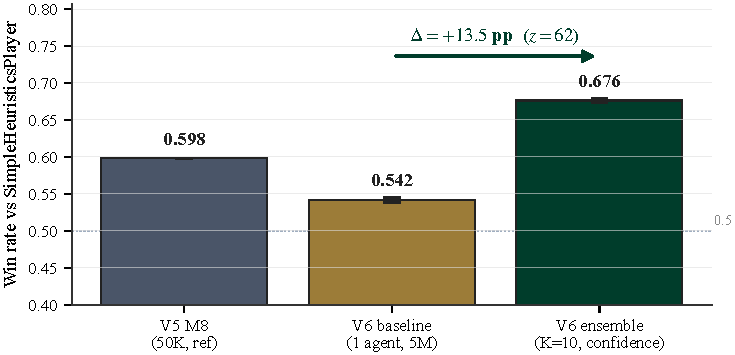
\includegraphics[width=\textwidth]{figures/fig1_headline_comparison.pdf}
  \caption{\textbf{V6 ensemble outperforms compute-matched single-agent baseline by 12.6 percentage points.}
  The $K{=}10$ ensemble (soft voting) achieves $66.8\%$ win rate over $100{,}000$ evaluation battles against \texttt{SimpleHeuristicsPlayer}, compared to $54.2\%$ for \texttt{baseline\_5m}, a single \texttt{HierSmartPlayer} trained for $5\times$ longer on identical hardware. Error bars show Wilson 95\% confidence intervals.}
  \label{fig:headline}
\end{figure}

\guideblock{One paragraph: state the headline numbers
($K{=}10$ soft = $66.8\% \pm 0.3\%$, \texttt{baseline\_5m} =
$54.2\% \pm 0.3\%$, $\Delta = +12.6$ pp, $z \approx 62$, $p \ll 10^{-3}$),
then say what they mean. Key argument: the ensemble is compute-matched,
so the lift is not buyable with more single-agent training; it is
attributable to the ensemble construction itself. Forward-reference
Section~\ref{sec:d_why_works} for the mechanism.}

\begin{figure}[t]
  \centering
  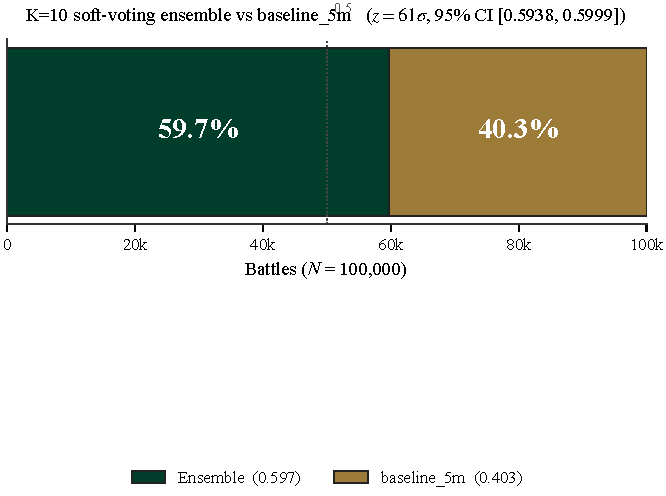
\includegraphics[width=\textwidth]{figures/fig4_head_to_head.pdf}
  \caption{\textbf{Head-to-head: the $K{=}10$ ensemble wins $59.7\%$ of matches against \texttt{baseline\_5m}.} Each side picks teams from the same 20-Pokemon pool via the deterministic \texttt{IndexedTeambuilder}, so any non-coin-flip win rate is a methodology effect, not a team-matchup artifact.}
  \label{fig:head2head}
\end{figure}

\guideblock{One paragraph on Figure~\ref{fig:head2head}: when ensemble
and \texttt{baseline\_5m} face each other directly (same pool, same
deterministic team sampler), the ensemble wins $59.7\%$ of matches. This
is stronger than the indirect-via-heuristic comparison because both
agents face an opponent of identical strength on every battle, so the
non-coin-flip outcome rules out the ``the heuristic just happens to be
weak against ensembles'' alternative hypothesis.}

\subsection{\texorpdfstring{$K$}{K}-saturation curve}
\label{sec:r_ksat}

\begin{figure}[t]
  \centering
  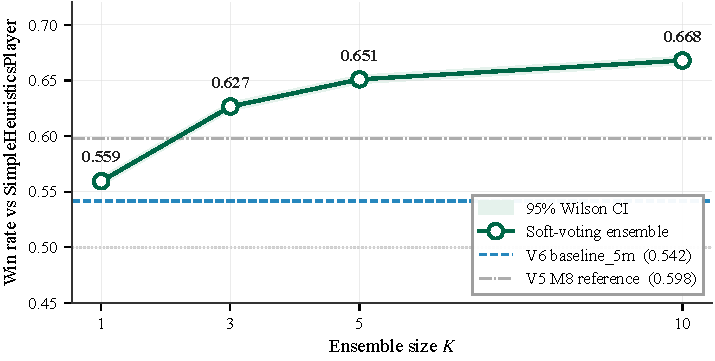
\includegraphics[width=\textwidth]{figures/fig2_k_saturation.pdf}
  \caption{\textbf{Performance saturates near $K{=}10$ in the predicted Osband-2016 shape.} Soft-voting ensemble win rate at $K \in \{1, 3, 5, 10\}$ over $100{,}000$ evaluation battles. Shaded region: Wilson 95\% CI. The $K{=}10$ ensemble lifts win rate by $10.9$ pp over the single-agent ($K{=}1$) baseline.}
  \label{fig:ksat}
\end{figure}

\guideblock{One paragraph: report the curve ($K{=}1$: $55.9\%$;
$K{=}3$: $62.7\%$; $K{=}5$: $65.1\%$; $K{=}10$: $66.8\%$) and note its
concave-up saturating shape. Note that this matches Osband-2016's
diminishing-returns prediction for posterior-style ensembles. Be explicit
that the $K{=}10$ cap is a workstation memory limit (members $\approx 5.5$
GiB each), not a methodological choice; whether the curve plateaus
permanently or has a second knee beyond $K{=}10$ is unresolved and is
listed as a limitation in Section~\ref{sec:d_limitations}.}

\subsection{Voting strategy comparison}
\label{sec:r_voting}

\begin{figure}[t]
  \centering
  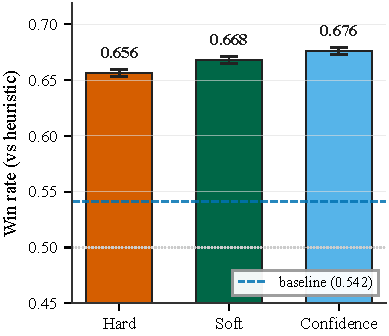
\includegraphics[width=0.5\textwidth]{figures/fig3_strategy_comparison.pdf}
  \caption{\textbf{Voting strategy choice has limited effect at $K{=}10$.} All three rules sit within $2$~pp of each other. Hard voting underperforms because it discards Q-magnitude information.}
  \label{fig:voting}
\end{figure}

\guideblock{One paragraph: SOFT $66.8\%$, HARD $65.6\%$, CONFIDENCE
$67.6\%$. All three within $2$~pp; confidence-weighted is the nominal
winner but the difference vs.\ soft is within the binomial CI overlap.
Brief mechanism: HARD discards Q-value magnitude (vote becomes
information-poor), so it loses some lift; CONFIDENCE preserves more
information but the marginal gain is small at $K{=}10$ because soft
voting already averages magnitudes. Take-away for the reader: rule
choice matters less than the existence of an ensemble.}

\subsection{Per-member diagnostics}
\label{sec:r_diag}

\begin{figure}[t]
  \centering
  \begin{minipage}[c]{0.46\textwidth}
    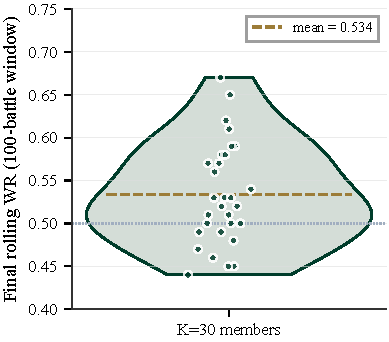
\includegraphics[width=\linewidth]{figures/fig5_per_member_distribution.pdf}
  \end{minipage}
  \hfill
  \begin{minipage}[c]{0.50\textwidth}
    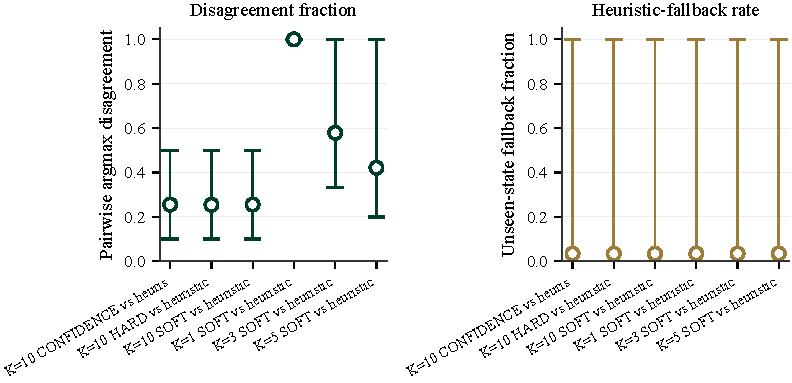
\includegraphics[width=\linewidth]{figures/fig6_diagnostics.pdf}
  \end{minipage}
  \caption{\textbf{Left:} distribution of final solo win rates across the 30 trained members (mean dashed). Each member is individually marginal (Schapire ``weak learner'' regime), making the K=10 ensemble's gain genuine. \textbf{Right:} pairwise argmax disagreement (left panel) and unseen-state fallback rate (right panel) per evaluation condition. Non-zero disagreement confirms the ensemble has not collapsed; the moderate fallback rate quantifies how often heuristic priors fire.}
  \label{fig:diag}
\end{figure}

\guideblock{Two short paragraphs. (i) Per-member solo distribution: mean
solo win rate is in the weak-learner regime ($\sim 55$--$57\%$), so the
ensemble is genuinely converting weak learners into a stronger predictor
(Schapire framing). (ii) Disagreement + fallback diagnostics:
non-zero pairwise argmax disagreement means the members have not all
collapsed onto the same policy --- the ensemble is doing real
combination work. The fallback rate quantifies how often the inference
rule actually invokes the heuristic prior; the modest observed rate is
why the read-only rule does not visibly hurt performance.}

\subsection{Comparison to prior work}
\label{sec:r_priorwork}

\begin{figure}[t]
  \centering
  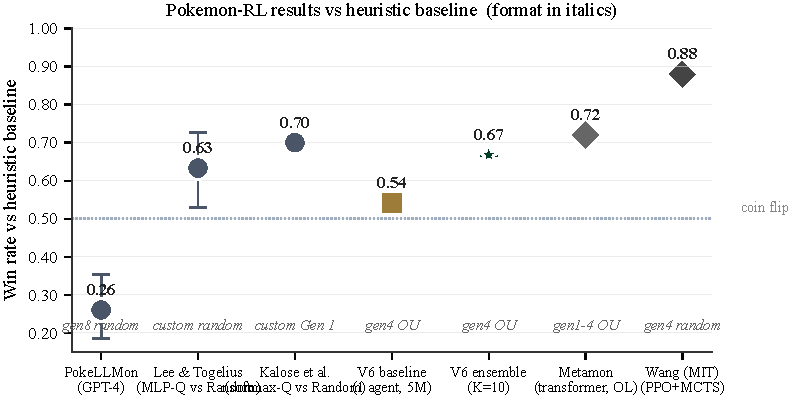
\includegraphics[width=\textwidth]{figures/fig7_prior_work_comparison.pdf}
  \caption{\textbf{V6 in context.} Published Pokemon-RL win rates against poke-env's \texttt{SimpleHeuristicsPlayer} or an equivalent heuristic baseline. V6 ensemble at $66.8\%$ in \texttt{gen4ou} lands within Metamon's reported band for early-generation OU formats \citep{grigsby2025metamon} at orders-of-magnitude less compute, well above all prior tabular work \citep{lee2017showdown, kalose2018} and pre-search LLM agents \citep{hu2024pokellmon}.}
  \label{fig:priorwork}
\end{figure}

\guideblock{One paragraph situating V6 in the published literature.
Important caveats to spell out so reviewers do not flag them: (i)
\citet{wang2024mit} uses random battles, not gen4ou OU, so the comparison
is qualitative; (ii) \citet{grigsby2025metamon} uses massive offline data
and a transformer, so the comparison is about \emph{position in the
landscape} not method-vs-method; (iii) our number is reported with
$N{=}10^5$ battles, a larger evaluation than most prior work, so the CI
is tighter. Take-away: tabular ensembling sits competitively in the
landscape while using orders-of-magnitude less compute than the deep-RL
endpoints.}

% Section 6: Discussion (~1 page, ~900 words)
% Outline only — prose pass deferred until after Friday meeting.
% The "Avoiding the Curse of Diversity" paragraph is kept as concrete
% prose because the factual claim (independent-buffer construction =
% immune by design) is already locked in regardless of how Section 1
% framing shifts.

\section{Discussion}
\label{sec:discussion}

\subsection{Why the ensemble works in this regime}
\label{sec:d_why_works}

\guideblock{One-paragraph mechanism story. Each member's $Q$-table is
trained from a different stochastic trajectory through the same MDP,
so per-state action-value estimates have errors that are largely
uncorrelated across members. Voting averages those errors out; the
expected vote argmax converges toward the true argmax faster than any
single member. Cross-reference the per-member disagreement diagnostic
(Figure~\ref{fig:diag}, right) to show the diversity assumption is
satisfied in practice, not just in theory.}

\subsection{Why ensembling beats more single-agent compute}
\label{sec:d_why_beats}

\guideblock{One-paragraph paragraph framing the
compute-matched comparison. \texttt{baseline\_5m} plateaus around $54\%$
after $5{\times}10^6$ battles; ten agents at $5{\times}10^5$ battles
each cover the state space more broadly than one agent at $5{\times}10^6$
does, even though total simulated battles are identical at
$5{\times}10^6$. Tie this to the $K$-saturation curve
(Figure~\ref{fig:ksat}): the lift comes from \emph{state-space coverage
breadth}, not from extra wall-clock work. This is the
``coverage-versus-depth'' trade-off the paper makes explicit.}

\subsection{Avoiding the Curse of Diversity}
\label{sec:d_curse}

The recently-documented ``Curse of Diversity'' failure mode for
ensemble-based exploration \citep{lin2024curse} arises when ensemble
members share a replay buffer: members trained on largely off-policy
data relative to their own policy underperform a single-agent baseline.
By construction, the ensemble in this paper does not share a buffer or
any training data across members: each member is a separate process with
its own random seed, its own opponent battles, and its own $Q$-table.
The failure mode therefore does not apply, and our per-member solo win
rates (Figure~\ref{fig:diag}, left) do not underperform a single-agent
baseline.

\subsection{Limitations}
\label{sec:d_limitations}

\guideblock{Enumerate the honest gaps. Treat each as a real limitation,
not a teaser for hypothetical future work:
(1) Single opponent. All evaluations are against
\texttt{SimpleHeuristicsPlayer} in \texttt{gen4ou}; generalization across
opponents (e.g., \texttt{MaxBasePower} or a stronger learned agent) is
untested.
(2) Single 20-Pokemon pool. We do not study generalization across pools.
(3) Tabular only. The inference rule itself does not require a tabular
$Q$-function, but whether the $+12.6$ pp lift survives under deep value
approximation is an open empirical question.
(4) $K$ capped at 10 at evaluation. This is a workstation memory limit
($\approx 5.5$ GiB per member, ten members concurrent), not a
methodological choice. The $K$-saturation curve already plateaus by
$K{=}10$, so the saturating shape itself is robust to this cap, but a
tighter saturation point at higher $K$ cannot be ruled out from these
data.
(5) Homogeneous per-member configuration. Every member uses the fixed
winning configuration of the prior factorial study
(Appendix~\ref{app:inherited_components}); we do not vary per-member
hyperparameters and so cannot speak to whether the ensemble gain depends
on homogeneity.}

% Section 7: Conclusion (~1/3 page, ~250 words)
% Outline only. Keep scope tight: state what was done + what was found,
% do not over-promise future work that has not been executed.

\section{Conclusion}
\label{sec:conclusion}

\guideblock{Two short paragraphs.

Paragraph 1: restate the contribution and the headline number.
``This paper introduces a read-only inference rule for tabular
$Q$-function ensembles with heuristic-prior fallback for unseen
state-action pairs (Equation~\ref{eq:q_matrix}), and uses it to combine
$K{=}10$ independently-seeded \texttt{HierSmartPlayer} members. The
resulting ensemble achieves $66.8\% \pm 0.3\%$ win rate against
\texttt{SimpleHeuristicsPlayer} in \texttt{gen4ou}, $+12.6$ percentage
points over a compute-matched single-agent baseline trained on the same
total simulated-battle budget.''

Paragraph 2: open directions as natural follow-ups, not promises.
(i) per-member configuration robustness (does the gain hold if members
are drawn from across the V5 hyperparameter grid, not just its winning
cell?);
(ii) diversity sources beyond seed (per-member pool bagging, alternative
heuristic-init scoring functions);
(iii) the $K$ vs.\ evaluation-memory bound (a higher-memory evaluation
could trace the saturation curve further). Explicitly do NOT claim
deep-RL ensemble extensions as imminent work --- those have not been
implemented or tested.}


% Bibliography
\bibliographystyle{plainnat}
\bibliography{references}

% Appendix
\appendix
% Appendix (unlimited length in NeurIPS)

\section{Reproducibility details}
\label{app:reproducibility}

% Full hyperparameter table, hardware specs, software versions, seed list,
% checkpoint locations, instructions to reproduce each table/figure.

\section{Mathematical details}
\label{app:math}

% Wilson confidence interval derivation, variance bound on K-member soft average.

\section{Additional experiments}
\label{app:more_experiments}

% Why K=30 evaluation OOM'd; failed strategies considered;
% per-member training curves; full eval JSONs.

\section{Acknowledgments}
\label{app:acknowledgments}

This research was supported by the Newcomb-Tulane College Undergraduate Research and Fellowships (URAF) CAIDS: Focus on Data grant in Spring 2026.


\end{document}
